% ============================================================
% FIGURES AND TABLES - as in the proposal: after the two pages of text,
% not counted in the page limit (to be confirmed by the professor).
% Every figure and table must be referred to in the text
% (e.g. Figure~\ref{fig:season-matched}) and have a self-contained caption.
% Each person adds their own figures here, in the order they are cited.
% ============================================================
\clearpage
\BAMunnumberedsection{Figures and Tables}
\label{sec:figures}

\begin{table}[H]
\centering
\small
\caption{Test performance on 2021--2022 (3{,}758 samples, 1{,}319 fires; random guessing gives AUPRC 0.351). AUPRC: area under the precision--recall curve; SM-AUPRC: season-matched AUPRC, with test non-fires reweighted to the fires' month distribution. F1 uses the threshold chosen without the test years. LR: logistic regression; RF: random forest; Month: a baseline that predicts each calendar month's fire rate in the training years and sees nothing else; Fusion: logistic-regression meta-learner on the RF and CNN probabilities, fitted on 2020.}
\label{tab:comparison}
\begin{tabular}{@{}lcccc@{}}
\toprule
Model & AUPRC & ROC-AUC & F1 & SM-AUPRC \\
\midrule
Month (baseline)         & 0.554 & 0.757 & 0.644 & 0.351 \\
LR            & 0.710 & 0.819 & 0.673 & 0.604 \\
RF            & 0.829 & 0.899 & 0.758 & 0.731 \\
CNN           & 0.749 & 0.843 & 0.695 & 0.705 \\
Fusion        & \textbf{0.864} & \textbf{0.917} & \textbf{0.780} & \textbf{0.793} \\
\bottomrule
\end{tabular}
\end{table}



% ---- Sophia ----
\begin{figure}[H]
    \centering
    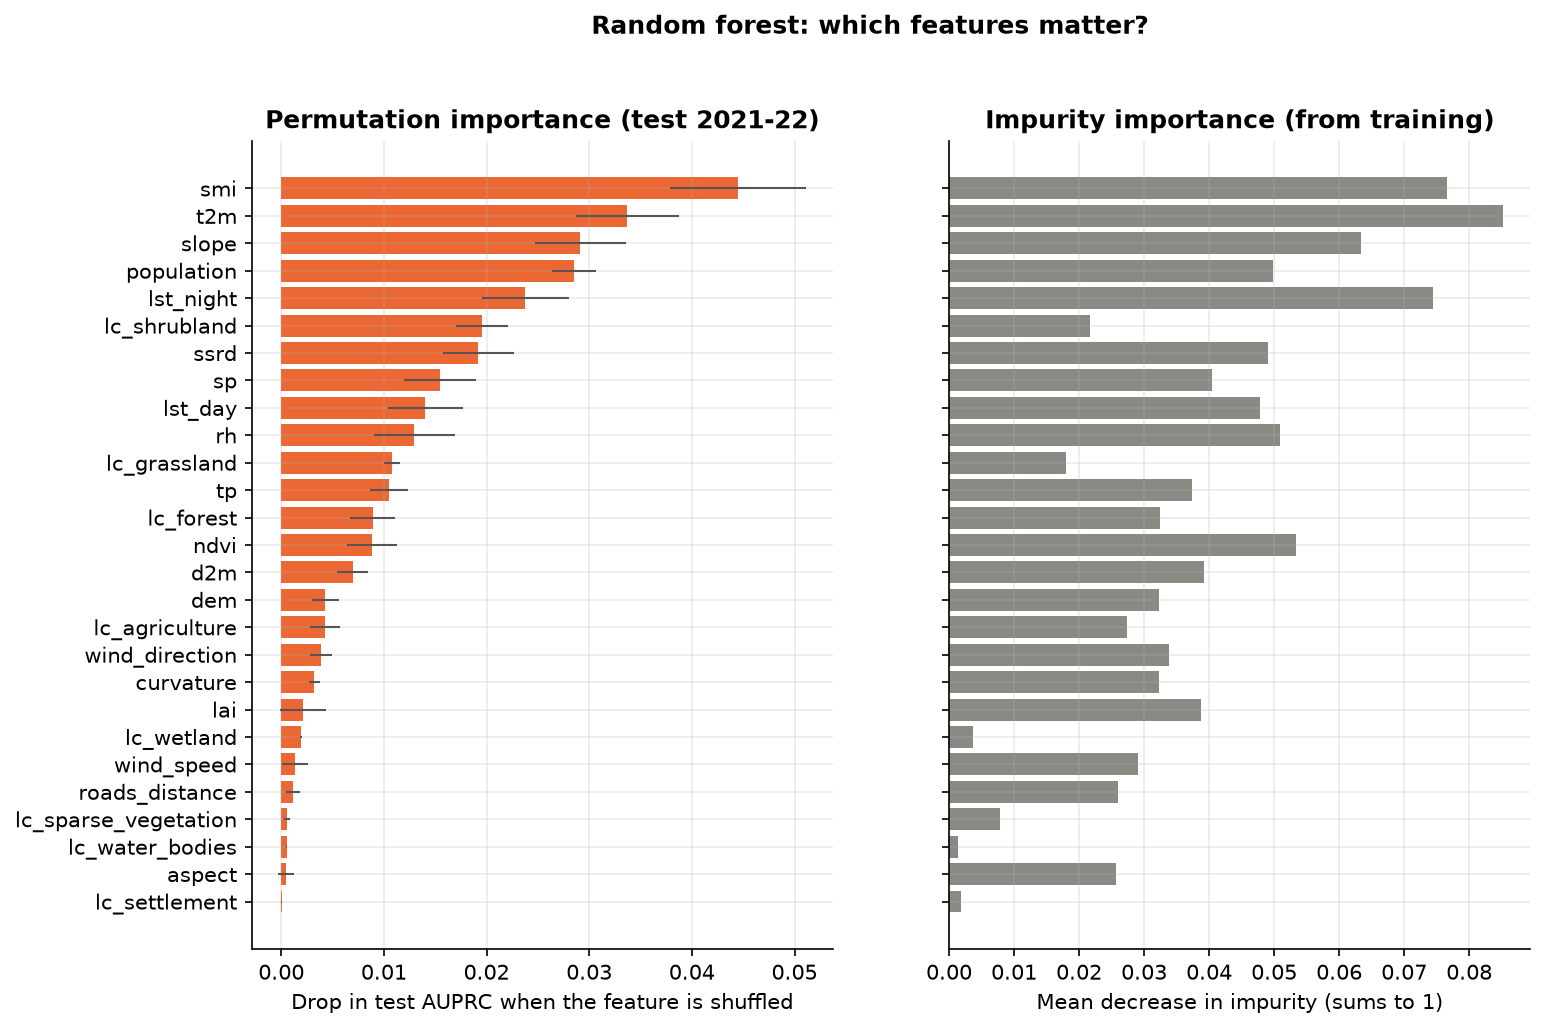
\includegraphics[width=0.85\linewidth]{sophia_rf_feature_importance.png}
    \caption{Random forest feature importance. Left: permutation importance, the drop in test AUPRC (2021--2022) when one feature's values are randomly shuffled; error bars show the spread over 10 shuffles. Right: impurity importance from training, shown for comparison. Soil moisture (smi), air temperature (t2m), slope, population and night-time land-surface temperature (lst\_night) matter most.}
    \label{fig:rf-importance}
\end{figure}

\begin{figure}[H]
    \centering
    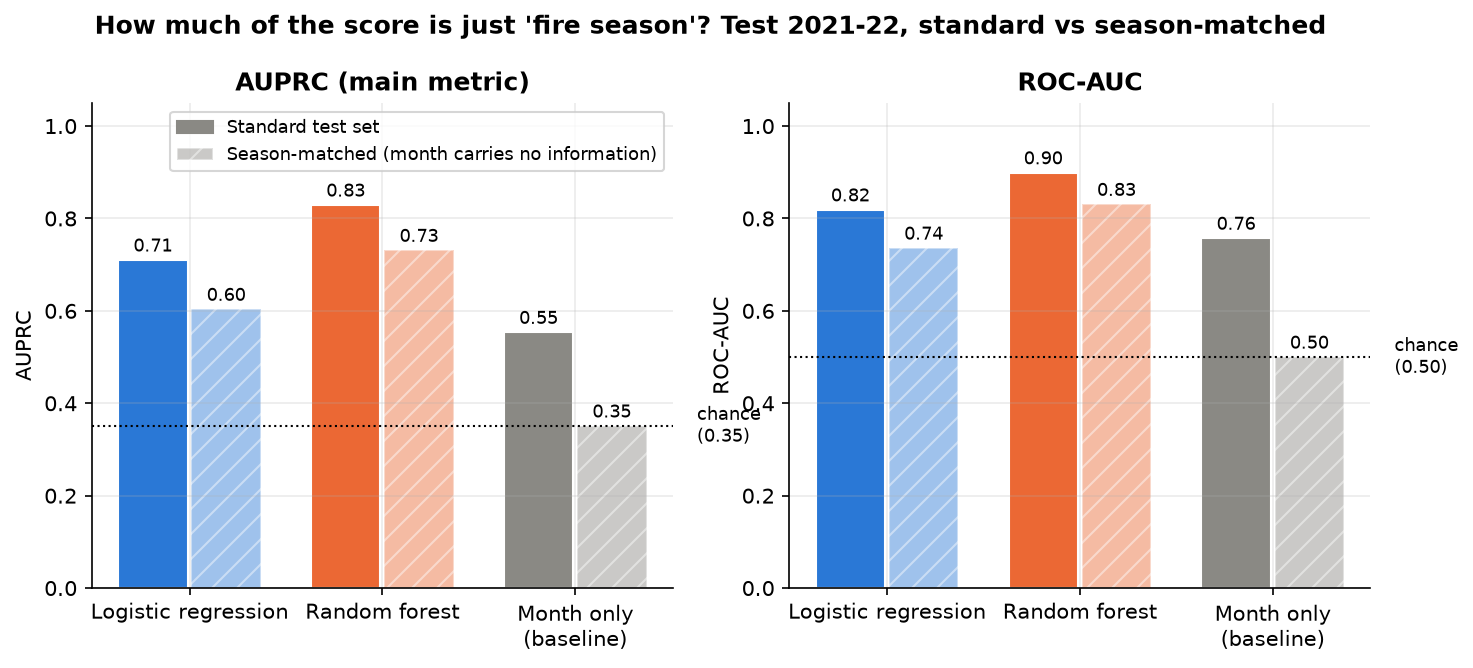
\includegraphics[width=0.85\linewidth]{sophia_season_matched.png}
    \caption{Test scores (2021--2022) of logistic regression, random forest and the month-only baseline, on the standard test set (solid) and season-matched (hatched), where non-fires are reweighted so the month carries no information. The dotted line is random guessing. The month-only baseline falls to chance under season matching, while both models stay well above it.}
    \label{fig:season-matched}
\end{figure}

% ---- Section 5 (comparison) ----
\begin{figure}[H]
    \centering
    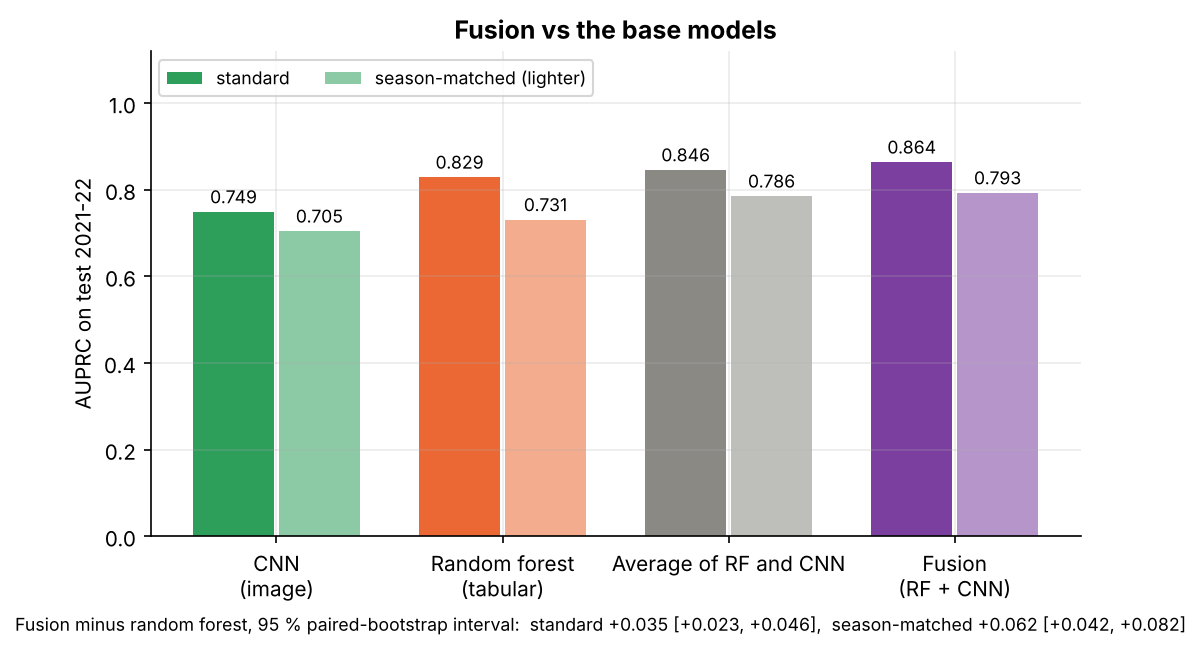
\includegraphics[width=0.85\linewidth]{claudia_fusion_auprc_bars.png}
    \caption{Test AUPRC (2021--2022) of the CNN, the random forest, a plain average of the two, and fusion, on the standard test set (dark) and season-matched (light). Fusion is best in both cases, and its gain over the random forest grows from +0.035 to +0.062 once the season effect is removed; the 95\% paired-bootstrap intervals (bottom) are well above zero.}
    \label{fig:fusion-bars}
\end{figure}

\begin{figure}[H]
    \centering
    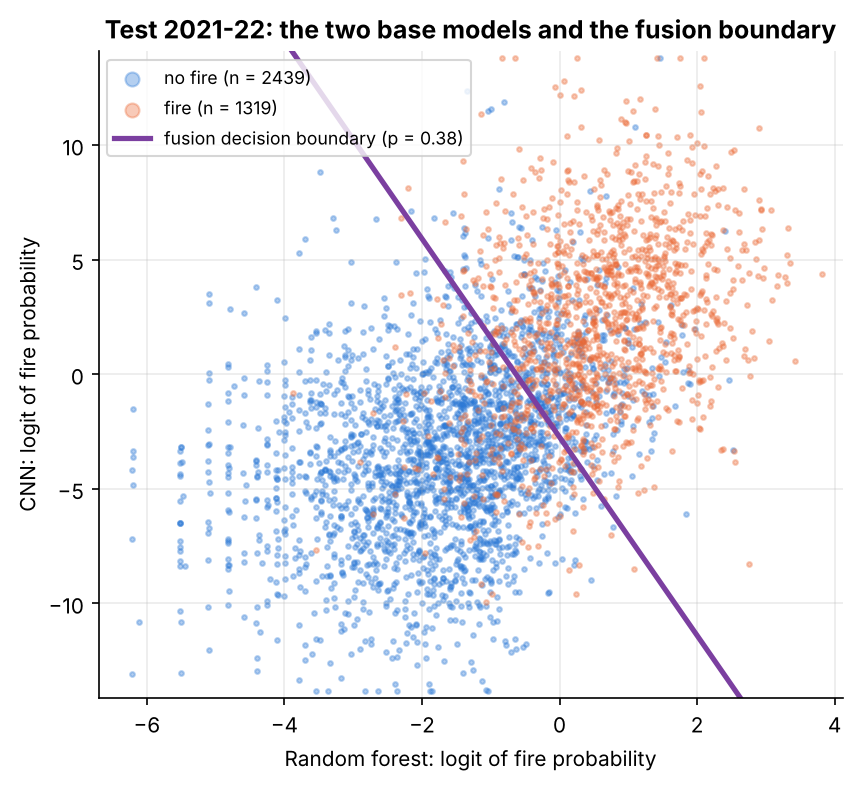
\includegraphics[width=0.7\linewidth]{claudia_fusion_scatter.png}
    \caption{Every test sample (2021--2022) placed by the random forest's prediction (x-axis) and the CNN's prediction (y-axis), both on the logit scale, coloured by the true label. Neither model alone separates fires (orange) from non-fires (blue), but together they do better: the tilted purple line is the fusion decision boundary.}
    \label{fig:fusion-scatter}
\end{figure}
% ---- Sandu: CNN figure (e.g. example tiles or training curve) ----
\begin{figure}[H]
    \centering
    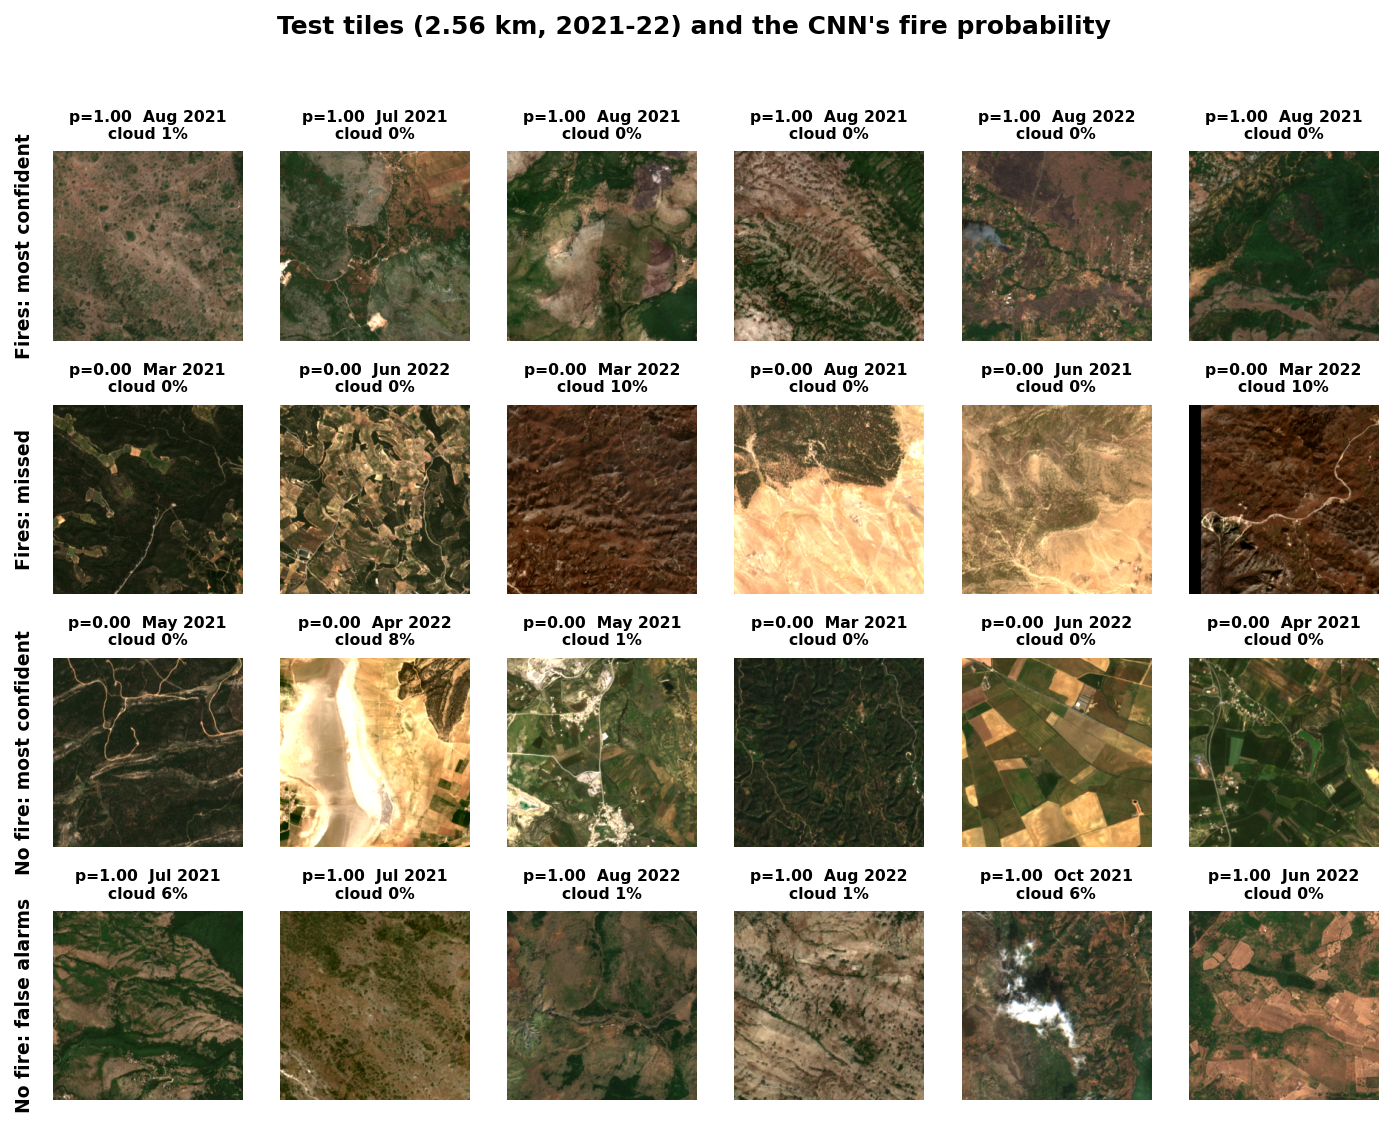
\includegraphics[width=0.85\linewidth]{sandu_example_tiles.png}
    \caption{An example of the Sentinel-2 test tiles from 2021-2022. Each tile captures an area of approximately 2.56\,km and was acquired 1-15 days before the fire day. Above each tile we have put the CNN's fire probability $p$, month of the scene and percentage of cloud coverage. The four rows show fires that the model was most confident about, some of the tiles it missed, where it was confident no fire would happen, and false alarms, where a fire was predicted but did not happen. The model separates dry and sparse land from dense forests, farmlands and water, therefore it recognizes fire prone places and not fire prone days.}
    
    \label{fig:cnn-tiles}
\end{figure}



\begin{figure}[H]
    \centering
    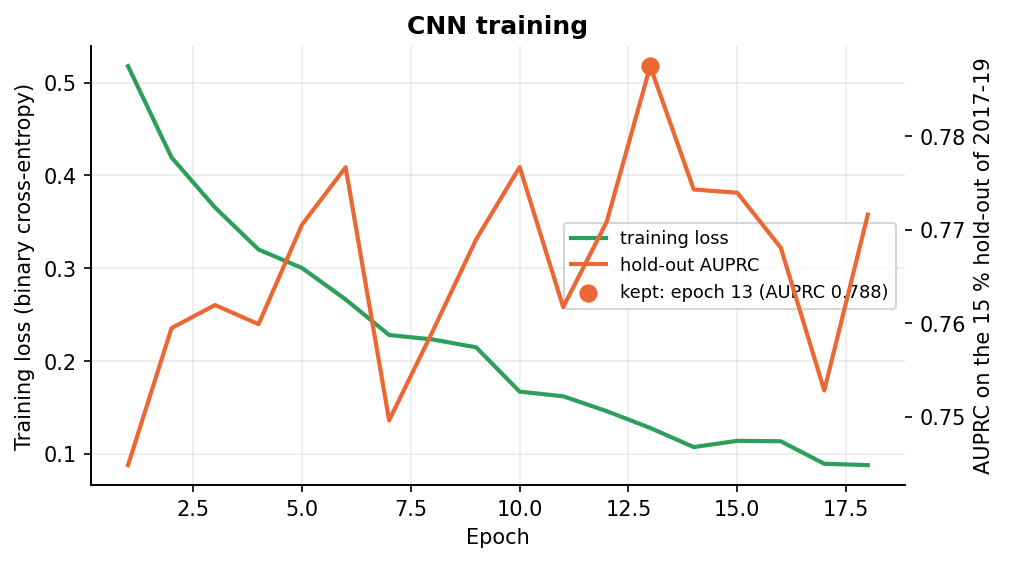
\includegraphics[width=0.75\linewidth]{sandu_training_curve.png}
    \caption{CNN training on 2017--2019: training loss (left axis) and AUPRC on the 15\,\% hold-out (right axis) per epoch. The loss keeps falling to 0.09 whilst the hold-out score flattens out at 0.75--0.79 from epoch 5 and all epochs afterwards, i.e.\ the network might memorise the training tiles without generalising better. Training was stopped after five epochs without improvement; the weights of epoch 13 were kept.}
    \label{fig:cnn-training}
\end{figure}

% ---- Claudia: fusion figure (e.g. fusion weights, or PR curves of all models) ----
% \begin{figure}[H]
%     \centering
%     \includegraphics[width=0.85\linewidth]{claudia_fusion.png}
%     \caption{[Self-contained caption.]}
%     \label{fig:fusion}
% \end{figure}
